\section{Data manipulation}
\label{sec:DataManipulation}
In the following subsections we describe different strategies for dataset manipulation from the most naive approach to more refined approaches such as trimming and analysis. These approaches are applied to the data before sending the input to the network. These strategies are used in experiments with the actual networks to locate the best possible strategy.

\subsection{Normalization}
For artificial neural networks to do the best work; the data should be normalized to either bipolar data [-1,1] or binary data [0,1]. This ensures the best performance by the activation functions since the sigmoid activation function has the steepest gradient (see figure ~\ref{fig:Sigmoid}) between -1 and 1 thus giving the finest granulated outputs. The same applies for the hyperbolic tangent(tanh) (see figure ~\ref{fig:Tanh}) activation function. The difference between the two are the output it generates from the same input. The hyperbolic tangent generates output that ranges from -1 to 1 and it has a steeper gradient around the y-axis than the sigmoid function thus giving the tanh function more granulated outputs than the sigmoid function.
\begin{figure}[H]
\centering
\begin{subfigure}{.5\textwidth}
  \centering
  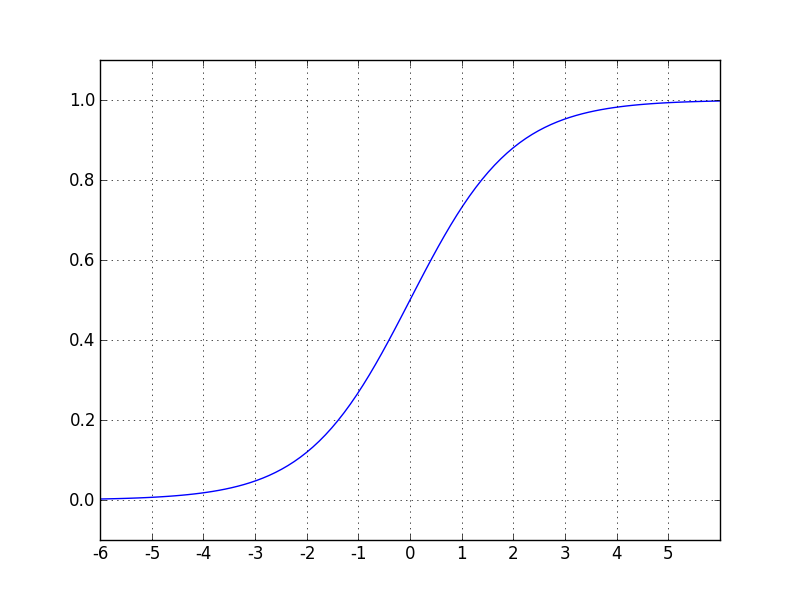
\includegraphics[width=\linewidth,natwidth=898,natheight=587]{billeder/activationFunctions/sigmoid.png}
  \caption{Sigmoid}
  \label{fig:Sigmoid}
\end{subfigure}%
\begin{subfigure}{.5\textwidth}
  \centering
  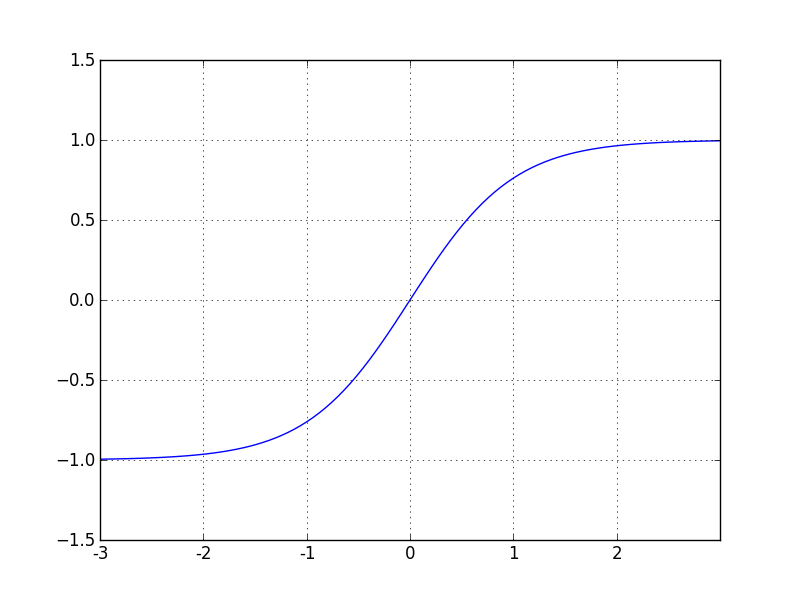
\includegraphics[width=\linewidth,natwidth=898,natheight=587]{billeder/activationFunctions/tanh.png}
  \caption{Hyperbolic tangent(tanh)}
  \label{fig:Tanh}
\end{subfigure}
\caption{Activation functions}
\label{fig:test}
\end{figure}

The normalization of the data is done using the following functions:
\begin{table}[H]
\centering  % used for centering table
\renewcommand{\arraystretch}{2}
\begin{tabular}{c c} % centered columns
 \#Normalization & \#Function \\ [0.5ex] % inserts table 
%heading
\hline                  % inserts single horizontal line
\multicolumn{1}{l}{Zero-to-one} & \multicolumn{1}{l}{$ X_{norm} = \frac{X_i - X_{min}}{X_{max} - X_{min}}$} \\
\multicolumn{1}{l}{Minus-one-to-one} & \multicolumn{1}{l}{$ X_{norm} = \frac{X_i - (\frac{X_{max} - X_{min}}{2})}{\frac{X_{max} - X_{min}}{2}}$} \\
[1ex]
\hline %inserts single line
\end{tabular}
\caption{Normalization functions} % title of Table
\label{table:naiveTrainingApproach} % is used to refer this table in the text
\end{table}
Where $X_i$ is the data entry, $X_{min}$ is the lowest value in the data set and $X_{max}$ is the highest value in the dataset.

%\subsection{The naive approach}
%The naive approach has almost no overhead and takes no preprocessing of the data. The method is simple; take one neuron per input and one neuron as output. Add all of the data to the training set without doing any preprocessing of data. This kind of training set is good enough for simple problems e.g. the XOR problem or likewise. When we talk about more complex real-world problems like forecasting the energy prices this method does not perform well. Another factor is that a huge %part of getting a neural network to perform well is the manipulation of the dataset to get rid of outliers and some of the noise in the dataset. Nevertheless it still gives an indication whether you have coherence between your input data and %the output data.

\subsection{Trimming}\label{sec:Trimming}
As mentioned before we need to get rid of some of the outliers and some of the noise in the data set to make it easier for the network to approximate a function based on the input data. There are different approaches to trimming but the two we use are standard trimming and percentile trimming of the dataset. Standard trimming is a simple way of getting rid of the worst outliers. The way to do it is; take a low and a high number in the dataset and remove everything below and above these limits. Of course this can be very arbitrary but with a simple plot diagram one will be able to see where the limits should be set. Percentile trimming is a statistic approach where the x\% of the dataset is removed from the top and the bottom. You make a percentage-wise distribution over the dataset; starting with the lowest values in the beginning and ending in the highest values. Then calculate the 1st percentile which represents the lowest 1\% of the dataset and then remove these values. The same is done for the top 1\% which results in the removal of the most extreme outliers and has made the dataset less error prone when doing statistical analysis on it. This method however only improves the predictions if the dataset contains extreme outliers. If none of the data falls in this category trimming might hurt the predictions more than improve them.

\begin{figure}[!ht]
\centering
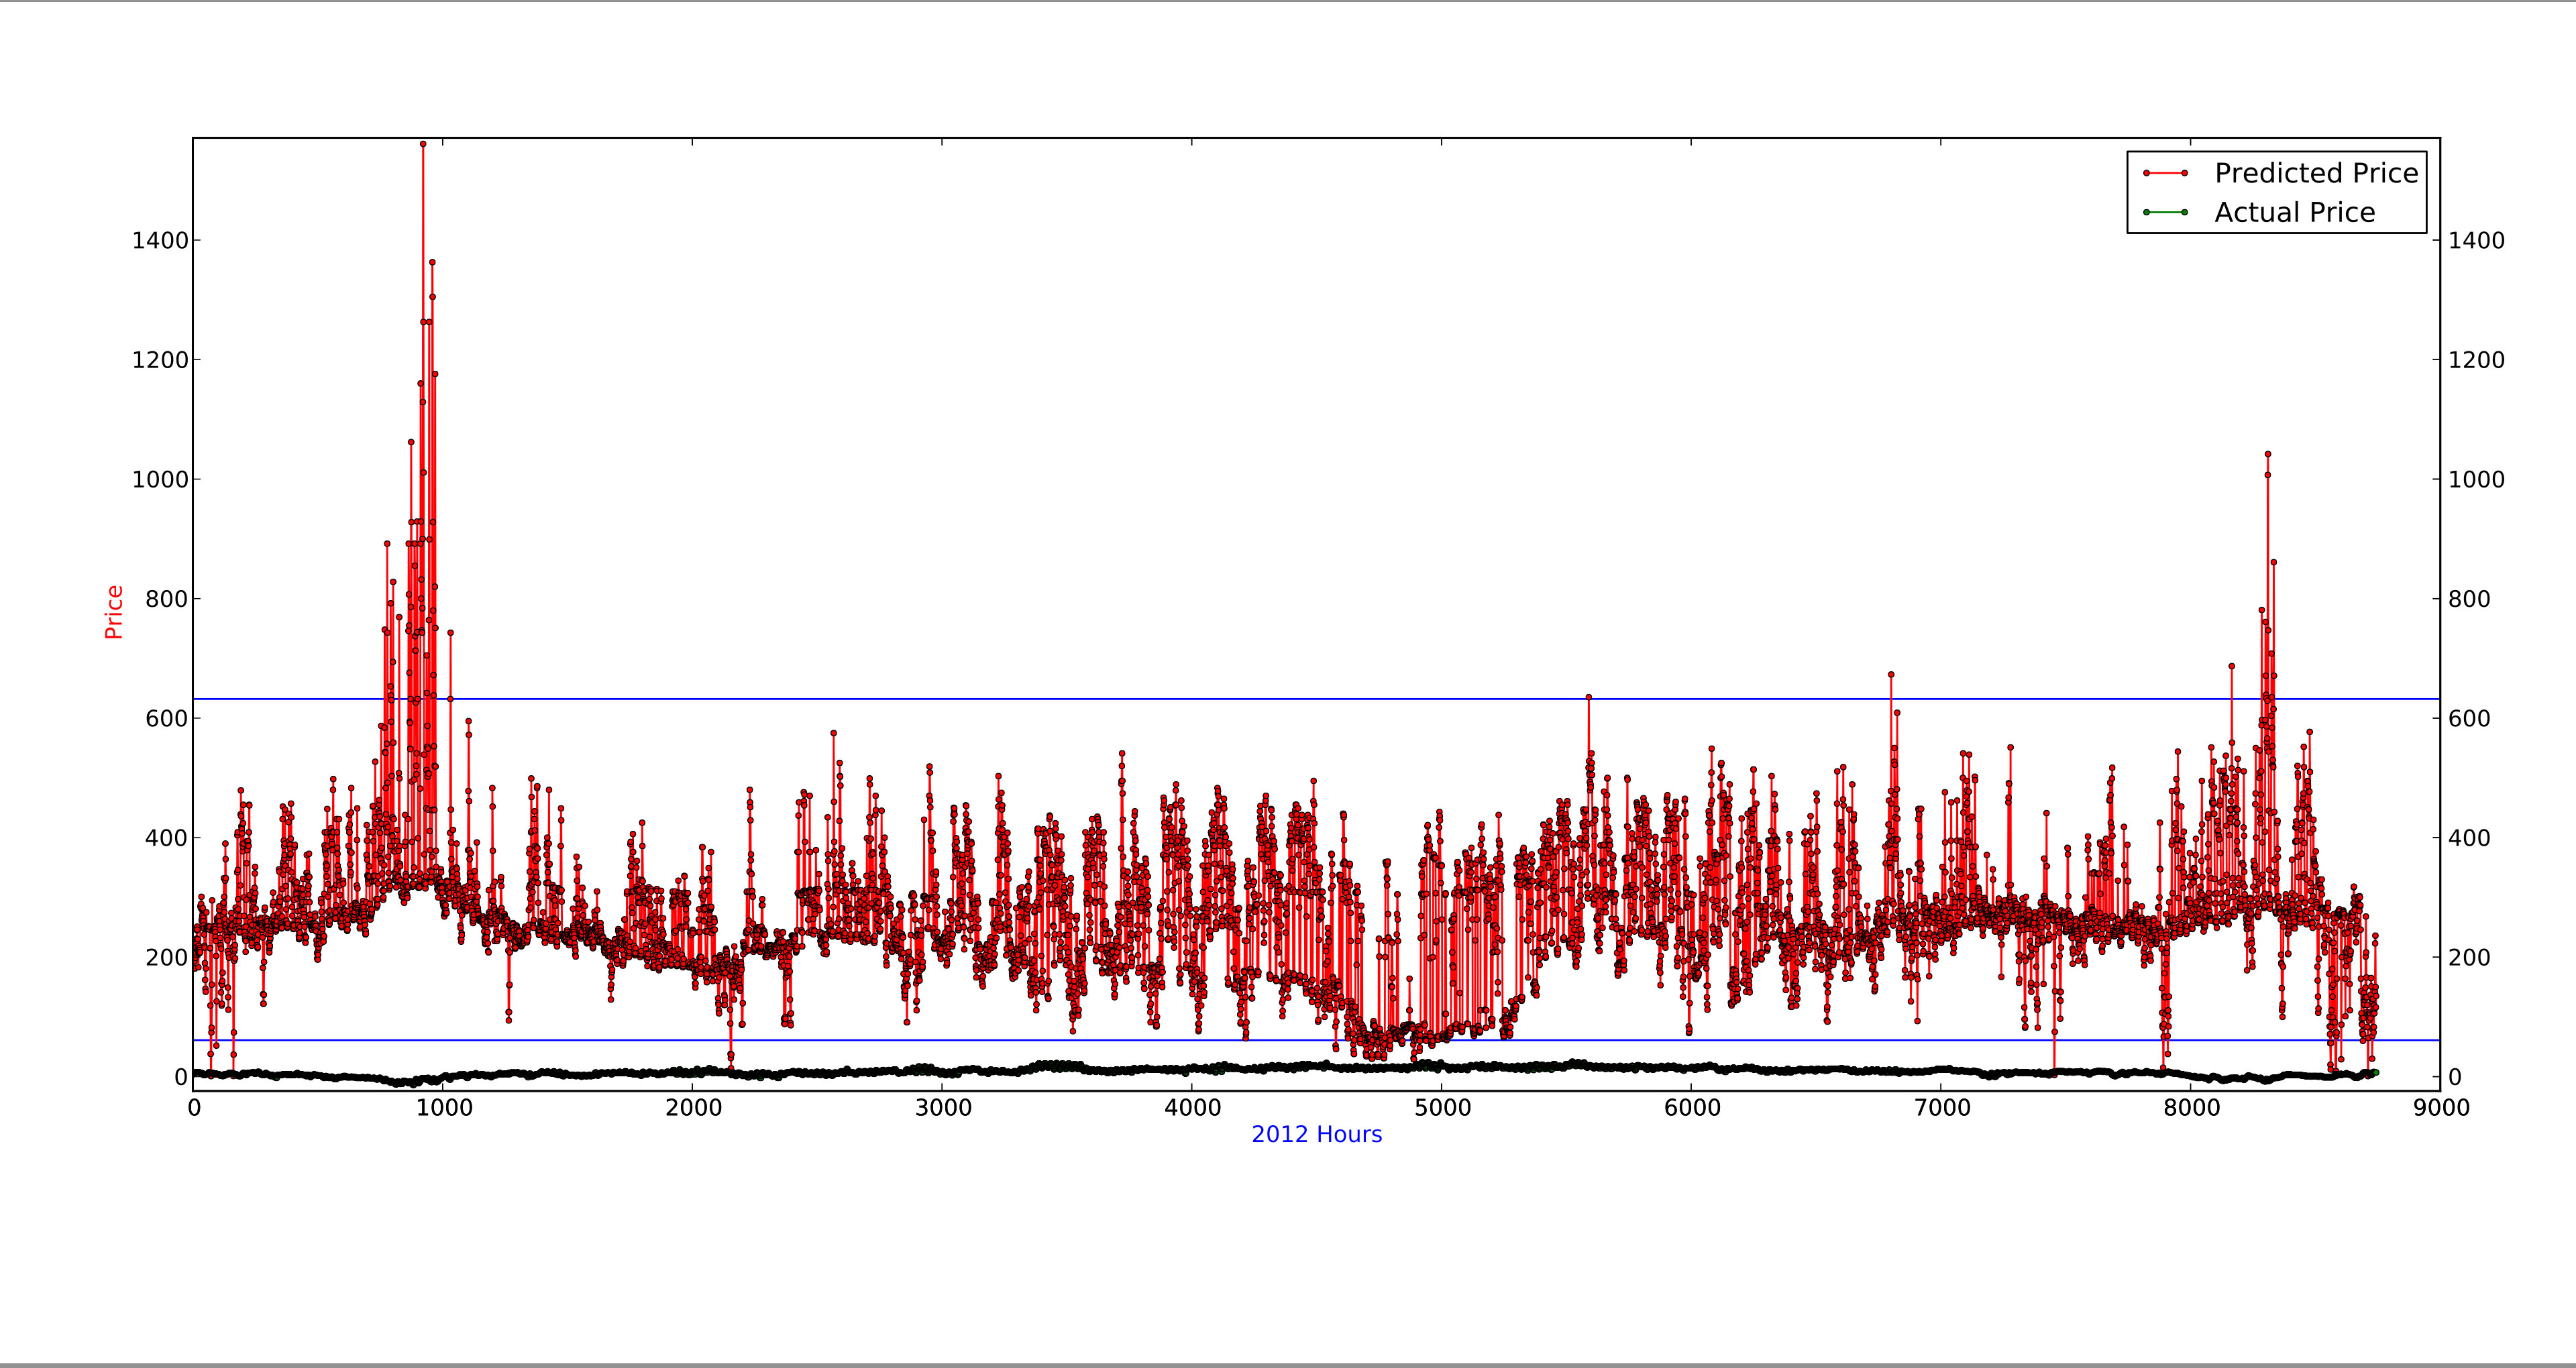
\includegraphics[width=\linewidth,natwidth=898,natheight=587]{billeder/trimming_graph.jpg}
\caption{This shows how trimming affects the prices of 2012. The blue lines show the upper and lower bounds of a 1\% trim.}
\label{fig:trimming_in_trimming_section}
\end{figure}

\subsection{Matrix}
\label{sec:Matrix}
\todo{Reference this articale: \cite{knerr1992handwritten}}
When analysing the data it is possible to find a connection between different rows of data e.g. what time of the day or what day of the week it is. These kind of data can be described using a single node where you normalize the hours by distributing them between -1 and 1. This will give this single neuron one weight to represent ALL of the values. One approach to give inputs more importance are by splitting them up into a simple matrix. This means that we for hours of the day have a matrix with one row and 24 inputs(one for each hour); we set a 1 in the input representing the time of day and set the rest to 0. This way the neural network will have a specific weight to apply according to which hour of the day it is and know exactly how each hour influence the output to predict. This of course adds a lot of overhead in terms of how many input nodes you need to have and how many nodes you need in the hidden layers. This will increase the processing time of the neural network iterations. This method is not only applicable for days. It can be applied to most inputs where you have a fixed and manageable sized set of different inputs to a single node. What can become a problem is if some values does not exist or are under-represented. This will cause that specific value to be under-expressed in the generalization thus not being able to cover these values if they should appear in the unseen data. The matrix manipulation makes the most sense when all values to some degree are equally distributed so that every input in the matrix can express all values equally. This is of course the case for hours of the day and months but a whole other story for wind speed. Wind speeds are in our dataset covered by 41 different values but these values are not necessarily equally distributed over an entire year. If one value is under-represented the network won't be able to express it generally. Take for instance if wind speed 5 is not represented in the training set, then the network will not be able to express it when encountering it in the unseen testing data.

\subsection{Historical Data}
\label{sec:historicalData}
It is the intention to achieve day-ahead forecasting by predicting the next 24 hours based on the past captured by the ANN as a generalization function  --- this can be defined as multiple step-ahead forecasting using an ANN\cite[Chapter~7.1.6]{econometrics}. 
If the analysis of a time series can identify trending behaviour then it will be of utmost importance for the forecast. The trends can be deterministic or stochastic but our time-series show stochastic properties since it at some time intervals will have a sequence of values that can lead to local trendlike movements\cite[Chapter~7.3]{econometrics}. Furthermore, it is necessary to investigate how to include this input information about the immediate past hours in order to give a better idea of what will come next. This will apply for the electricity prices but also to some extend the wind production since it follows consumption (Section~\ref{sec:consumptionWindProduction}). It points us in the direction of simple slope calculation or statistics used in economy to capture trends of the immediate past and use it as input. The concrete methods will be discussed in more detail in sections to come. The purpose of using the slope as input would be to have an indicator of which way we are moving, up or down. This can be made more sophisticated by using actual statistics for gathering some of the price characteristics (Presented at~\ref{sec:electriciyPrices}) like frequency, seasonality and volatility. It could also be an option to include past prices as input parameters to include the historical perspective as presented in \cite{singhal2011electricity}.
What is evident is the need for analysing the price and wind production curves both to capture the tendencies but at the same time locating irregularities --- prices or productions that are so obscure that we won't be able to predict them. Experiments with the different approaches will be conducted.
